\chapter{TELEVISIÓN DIGITAL TERRESTRE DVB-T1}
\section{Introducción}

Ideas a incluir en la introducción:

\begin{itemize}
    \item En 1950 la televisión a blanco y negro analógica comenzó a extenderse por el mundo y convertirse en uno de los eventos más memorables. En ese momenot ya se había extendido el uso del teléfono, pero resultaba muy costoso usarlo en llamadas de larga distancia.
    \item Pero ya desde 1948, Shannon ya estaba comenzando a usar la palabra bit para llegar a producir la revolución digital que estamos viviendo hoy, donde la información fluye en forma digital por cables o sin ellos.
    \item En ese momento, la tecnología digital parecía algo innecesario ya que por un lado significaba tecnología más costosa y por el otro requería mayores anchos de banda. 
    \item En realidad, la tecnología digital tiene sus desventajas, pero las ventajas son mayores. El progreso que ha habido en la electrónica, pero también en las técnicas de codificación del canal y en algoritmos de procesamiento digital han sido claves para que las comunicaciones digitales se impongan.
\end{itemize}

\section{Conceptos previos}

\subsection{Polinomio generador de código}

Cualquier código binario puede ser representado mediante un determinado polinomio G(x), de cierto grado r. También puede decirse que cualquier polinomio de estos puede generar un código binario, por eso se habla de un polinomio generador Por ejemplo, el Polinomio Generador podría ser. 

\begin{equation} \label{capsiete_uno}
G(x)=x^{3}+1, el \ cual \ es \  de  \ grado \ es \ r=3
\end{equation}


\begin{equation} \label{capsiete_dos}
G(x)= 1x^{3}+0 x^{2}+0 x +1x^{0}
\end{equation}

El código binario corresponde a los coeficientes: 1001 
Los signos de suma en los polinomios generadores son suma por módulo 2. Por eso podríamos decir que $X^{2}+X^{2}=0, ya \ que 1 \oplus 1 \rightarrow 0.$


\section{Aritmética de módulo 2}

Vale la pena recordar la aritmética de módulo 2, donde las sumas y las restas funcionan como compuertas XOR.\\


\begin{equation} \label{capsiete_tres}
0 \oplus 0 \rightarrow 0
\end{equation}

\begin{equation} \label{capsiete_cuatro}
1 \oplus 0 \rightarrow 1
\end{equation}

\begin{equation} \label{capsiete_cinco}
0 \oplus 1 \rightarrow 1
\end{equation}

\begin{equation} \label{capsiete_seis}
1 \oplus 1 \rightarrow 0
\end{equation}

\subsection{Campos de Galois}

\section{Fundamentos de codificación del canal}

\subsection{Teorema de Shannon}

Ideas a incluir en este capítulo:
\begin{itemize}
    \item El Teorema de Shannon o Teorema de codificación del canal ruidoso establece las fronteras para la máxima información teórica que se puede transferir a un canal con un cierto nivel de ruido. 
    \item Increíblemente, los últimos límites en la teoría de la información y codificación fueron determinados justo cuando esta ciencia nació, con los primeros artículos de Shannon.
    \item El resultado más conocido de Shannon es el teorema de la capacidad de un canal. El teorema establece que para muchas clases comunes de canal existe un parámetro que ha sido llamado Capacidad de Canal C, sobre el cual viajan códigos a una rata R<C que pueden alcanzar transmisiones con cualquier grado de confiabilidad, pero estos códigos no existen para R>C.
    \item El teorema también establece que para una canal de ancho de banda B (Hz) y afectado solo por ruido blanco aditivo gaussiano (AWGN del inglés Additive White Gaussian Noise), la capacidad C (en bps) solo depende de dos parámetros: el ancho de banda B y la relación señal a ruido SNR (del inglés Signal to Noise Relationship), así. 
    
    \begin{equation} \label{capsiete_siete}
   C = Blog_{2}(1+ SNR)
    \end{equation}
    
    \item Este teorema ha significado un reto para las siguientes generaciones de investigadores que se han enfrascado en lograr que sus algoritmos se acerquen al menos a ese límite establecido por Shannon. En los procesos de codificación y decodificación está en gran manera la clave para alcanzarlo. 
\end{itemize}

\subsection{El proceso de codificación y decodificación digital del canal}

El problema de la codificación es planteado por el canal. Como ya  se ha dicho en otros capítulos los efectos del canal en el proceso de la comunicación es la razón por la cual aumenta constantemente el número de elementos o nuevos métodos de tratamiento de la información. Pareciera que con lo visto en capítulos anteriores, ya se ha visto todo sobre esos métodos, pero la realidad es que por más soluciones que se implementen siempre existirá la posibilidad de que la información llegue al destino con errores.

\vspace{200px}
\begin{figure}[h!]
	\captionsetup{justification = raggedright, singlelinecheck = false}
	\caption{Ruta de recepción de un mensaje.} 
	\centering
	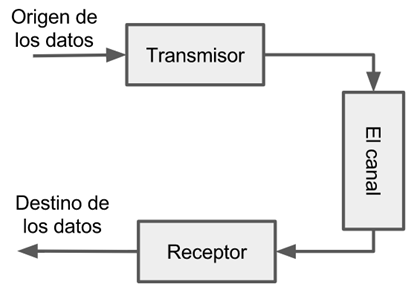
\includegraphics[scale=1]{Imagenes/Origen-datos.png}
	\label{fig:Origen-datos}
	%		\captionsetup{justification=raggedright,font={scriptsize,bf,it}}
	%		\caption*{fuente: http://superkuh.com/rtlsdr.html}
\end{figure}

Entonces surgen varias preguntas:
\begin{itemize}
    \item ¿Es posible reconocer en qué momento se están presentando los errores?
    \item ¿Qué acciones es posible tomar cuando se han detectado errores?
\end{itemize}
La solución a estas preguntas está en lo que se conoce como Codificación del Canal. La idea es enviar junto con la información ciertos datos adicionales que permitan detectar la pérdida de bits, lo cual llamaremos codificación y se realiza en el transmisor. Finalmente, en el receptor se debe realizar el proceso de la detección de los errores, su corrección y la decodificación para recuperar los datos enviados, como se muestra en la siguiente figura. \\

\begin{figure}[h!]
	\captionsetup{justification = raggedright, singlelinecheck = false}
	\caption{Proceso de codificación } 
	\centering
	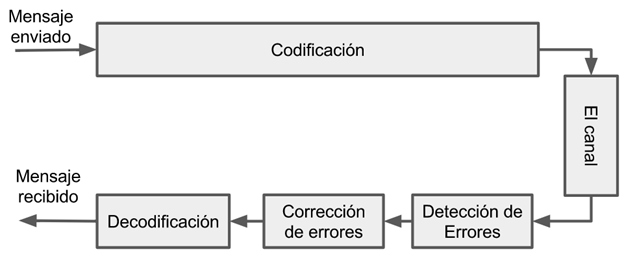
\includegraphics[scale=1]{Imagenes/Proceso-deco.png}
	\label{fig:Proceso-deco}
	%		\captionsetup{justification=raggedright,font={scriptsize,bf,it}}
	%		\caption*{fuente: http://superkuh.com/rtlsdr.html}
\end{figure}


\subsection{Los retos de la teoría de codificación del canal}

El primer reto consiste en poder corregir el máximo número de errores mientras se usa la mínima redundancia (rata) posible
El segundo reto consiste en construir códigos que tengan procesos eficientes de codificación y decodificación

\section{Códigos de Repetición}

\subsection{El Código de Repetición (3,1)}

Para presentarle rápidamente un ejemplo de codificación al lector, a continuación se analiza el ejemplo más sencillo de codificación. Consiste en transmitir 3 veces cada bit. 
Entonces se tiene una tabla de verdad, a la cual también se refieren como un diccionario

	\begin{table}[h!]
		\captionsetup{justification = raggedright,singlelinecheck = false}
		\caption{Alguna descripción.}
		\label{tabla:tabla12}
		\centering
		\scalebox{1}{
		\begin{tabular}{|c|c|}
			\hline
			\textbf{Bit de información} &\textbf{Palabra asignada} \\ \hline
			0 & 000  \rule[1mm]{0mm}{5mm}\\ \hline 
			1 & 111  \rule[1mm]{0mm}{5mm} \\ \hline
		\end{tabular}}
	\end{table}
	
En el receptor, para el ejemplo dado, se pueden recibir 8 posibles versiones de datos a interpretar. En el receptor podría usarse la siguiente tabla de verdad para interpretar la información útil:

	\begin{table}[h!]
	\captionsetup{justification = raggedright,singlelinecheck = false}
	\caption{Alguna descripción.}
	\label{tabla:tabla13}
	\centering
	\scalebox{0.90}{
		\begin{tabular}{|c|c|c|}
			\hline
			\textbf{Tribits recibidos} & \textbf{Bit Interpretado} & \textbf{Número de Errores identificados} \\ \hline
			000 & 0 & 0  \rule[1mm]{0mm}{5mm}\\ \hline 
			001 & 0 & 1  \rule[1mm]{0mm}{5mm} \\ \hline
			010 & 0 & 1	 \rule[1mm]{0mm}{5mm} \\ \hline
			100 & 0 & 1	 \rule[1mm]{0mm}{5mm} \\ \hline
			111 & 1 & 0  \rule[1mm]{0mm}{5mm} \\ \hline
			110 & 1 & 1  \rule[1mm]{0mm}{5mm} \\ \hline
			101 & 1 & 1  \rule[1mm]{0mm}{5mm} \\ \hline
			011 & 1 & 1  \rule[1mm]{0mm}{5mm} \\ \hline
			
	\end{tabular}}
\end{table}

\textbf{Ventajas de esta codificación:} es muy fácil codificar y decodificar\\

\textbf{Desventaja:} Baja rata $ \frac{1}{3} $\\
Un vídeo explicativo es el siguiente:
\textcolor{blue}{\href{https://www.youtube.com/watch?v=0CLTy231Hsw}{Vídeo }}

\subsection{ El Código de repetición basado en una matriz 2x3}

El código se obtiene a partir de una matriz G
Por ejemplo 
\begin{equation} \label{capsiete_ocho}
G= \left(
\begin{array}{lcr}
1 & 0 & 1 \\
0 & 1 & 1 \\
\end{array}
\right)
\end{equation}

Como la matriz es de dimensión 2x3, el el mensaje se organiza en bloques de a 2 bits o símbolos.

\begin{equation} \label{capsiete_nueve}
m= {\mu_{1}, \mu_{2}} 	\in  F^{2}
\end{equation}

Mediante una multiplicación matricial se obtiene la señal a transmitir.

\begin{equation} \label{capsiete_diez}
T= m / x / G
\end{equation}

Para el ejemplo

\begin{equation} \label{capsiete_once}
T \ = \ ({\mu_{1}, \mu_{2}})  \left(
\begin{array}{lcr}
1 & 0 & 1 \\
0 & 1 & 1 \\
\end{array}
\right) ({\mu_{1}, \mu_{2}, \mu_{1} + \mu_{2} })
\end{equation}

como el último componente es la suma de los dos primeros, este puede indicar si hay o no error, por ejemplo si $u_{1}=1$, $u_{2}=1$, entonces  para el último miembro debe ocurrir que $u_{1} \oplus u_{2} = 0$. \\

El código es el conjunto de todas las posibles combinaciones de símbolos a transmistir. Para el ejemplo dado el código tiene 4 posibles palabras, pues al organizar la información por dibits, se tendrán $2^{2}=4$ posibles dibits diferentes. Para este ejemplo, también se dice que T pertenece a un espacio $F_{2}^{3}$ . Eso significa que en ese espacio pueden haber $2^{3}=8$ posibles combinaciones, pero que solo 4 son de información válida. \\

La ventaja con respecto al código del capítulo anterior, es que por cada 2 componentes del mensaje se envía en 3 elementos, entonces la Rata es $\dfrac{2}{3}$ La desventaja: se puede detectar 1 error, pero no se puede corregir.

\section{Principales parámetros de la codificación}

\subsection{ Distancia de Hamming entre dos palabras}

Se usa normalmente para comparar una palabra digital original con respecto a otra que puede ser una versión codificada o una versión recibida con errores. La distancia de Hamming es el número de bits que difieren en esas dos palabras. En la figura \ref{fig:Unos-ceros} se muestran dos palabras a comparar.

\begin{figure}[h!]
	\captionsetup{justification = raggedright, singlelinecheck = false}
	\caption{Comparación entre dos palabras.} 
	\centering
	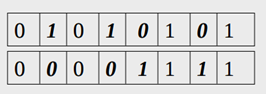
\includegraphics[scale=1]{Imagenes/Unos-ceros.png}
	\label{fig:Unos-ceros}
	%		\captionsetup{justification=raggedright,font={scriptsize,bf,it}}
	%		\caption*{fuente: http://superkuh.com/rtlsdr.html}
\end{figure}

En ellas, la distancia de Hamming es 4, lo cual significa que se necesitan 4 errores para transformar una palabra en la otra. La manera en que se simboliza matemáticamente la distancia de Hamming es la siguiente: \\

\begin{center}
    d(101101, 110100) = 3
\end{center}

Significa que la distancia entre los códigos 101101 y 110100 es 3.\\

\subsection{Distancia de Hamming de un código}

Supongamos que se desea emitir un mensaje que solo tiene las vocales abiertas: a,e,o. De manera que a cada vocal le asignamos un código, entonces tenemos por ejemplo las siguientes tres palabras {100, 111, 011}. Para cada pareja de palábras de un código se pueden tener diferentes distancias, para este ejemplo tenemos:\\

d(100,111)=2 \\

d(100,011)=3 \\

d(111,011)=1 \\

La Distancia de Hamming para el código dado, de varias palabras es el mínimo de todas las distancias. Para el ejemplo dado es 1. Es claro que entre más grande sea esta distancia, mejor será el código, pues es más grande la diferencia entre las palabras, de modo que los errores que puedan resultar son más fácilmente identificables.\\

Veamos un ejemplo de codificación usando una matriz 3x6.\\

\begin{itemize}
    \item El mensaje binario se divide en bloques de 3 bits, de manera que uno de esos bloques podría representase mediante un símbolo m, por ejemplo:
    \begin{equation} \label{capsiete_doce}
    m = [110] \in F^{3}  
    \end{equation}
     \item La matriz de codificación a usar es la siguiente:
    \begin{equation} \label{capsiete_trece}     
G= 
\begin{bmatrix}
    1 & 0 & 0 & 1 & 1 & 0 \\
    0 & 1 & 0 & 1 & 0 & 1 \\
    0 & 0 & 1 & 0 & 1 & 1 \\
\end{bmatrix}
    \end{equation}
    
    \item La señal a transmitir sería entonces $T \ = \ u \ x \ G$. \\
    Ejemplo para los simbolos 110 y 101.
    
        \begin{equation} \label{capsiete_catorce}     
(1,1,0)
\begin{bmatrix}
    1 & 0 & 0 & 1 & 1 & 0 \\
    0 & 1 & 0 & 1 & 0 & 1 \\
    0 & 0 & 1 & 0 & 1 & 1 \\
\end{bmatrix} = (1,1,0,0,1,1)
    \end{equation}

        \begin{equation} \label{capsiete_quince}     
(1,0,1)
\begin{bmatrix}
    1 & 0 & 0 & 1 & 1 & 0 \\
    0 & 1 & 0 & 1 & 0 & 1 \\
    0 & 0 & 1 & 0 & 1 & 1 \\
\end{bmatrix} = (1,0,1,1,0,1)
    \end{equation}
\end{itemize}

Podríamos hacer lo mismo para $2^{3}=8$ palabras, se dice que el código pertenece a un $F_{2}^{6}$, es decir un espacio que tiene $2^{6}=64$ posibles elementos, pero sólo $2^{3}=8$ son parte del código.
Si realizamos el análisis para todas las posibles palabras, descubriremos que la distancia de hamming es igual a 3, pues al menos 3 bits serán diferentes entre cualquiera de las componentes del código.
Si una palabra de un código C se representa como x y otra como y, se dice que la distancia de Hamming es:
h(x,y)= el número de símbolos de x que diferente de y
y para todo un código C, la distancia es: 

\begin{equation} \label{capsiete_diesiseis}
d(C) = min \ {h(x,y) \ | \ x,y \in C,x 	\neq y }
\end{equation}

Podemos imaginar que el campo $F_{2}^{6}$  es el que se presenta en la siguiente figura.

\vspace{200px}
\begin{figure}[h!]
	\captionsetup{justification = raggedright, singlelinecheck = false}
	\caption{El espacio $F_{2}^{6}$ Los puntos negros representan las posibles palabras que pueden resultar en el campo y los círculos representan las palabras del código} 
	\centering
	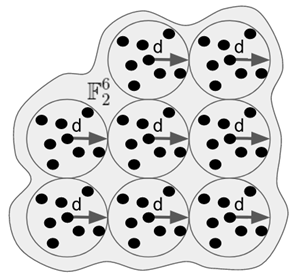
\includegraphics[scale=1]{Imagenes/Espacio.png}
	\label{fig:Espacio}
	%		\captionsetup{justification=raggedright,font={scriptsize,bf,it}}
	%		\caption*{fuente: http://superkuh.com/rtlsdr.html}
\end{figure}

En la gráfica podemos observar que cada palabra del código tiene una cobertura de radio d. Quiere decir que si al receptor llega la señal con errores, en todo caso cada palabra recibida caerá dentro del área de cobertura de una palabra del código y es lo que permitirá corregir el error. Por eso es importante que el código cuente con coberturas grandes, que abarquen todo el espacio. \\

La gráfica anterior se refuerza si observamos que un bloque (n,k), que es un código C(n,k) y proviene de una matriz G de n x k, es un subespacio de un espacio vectorial $F^{n}$ y las filas de G son la base de C.

\subsection{La rata del código.}

En cualquier caso de codificación se tiene un mensaje de k que luego de la codificación sale con n palabras.

\begin{figure}[h!]
	\captionsetup{justification = raggedright, singlelinecheck = false}
	\caption{Rata del código.} 
	\centering
	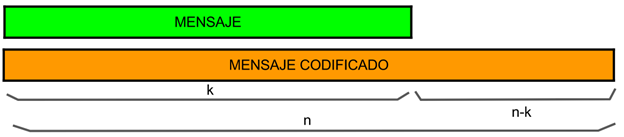
\includegraphics[scale=1]{Imagenes/Mensaje.png}
	\label{fig:Mensaje}
	%		\captionsetup{justification=raggedright,font={scriptsize,bf,it}}
	%		\caption*{fuente: http://superkuh.com/rtlsdr.html}
\end{figure}

La rata de codificación Rc señala qué tan eficiente es el código en términos de la cantidad de información redundante que es necesario transmitir.

\begin{equation} \label{capsiete_diesisiete}
Rc = \dfrac{k}{n}
\end{equation}

\subsection{La ganancia del código}

Es la diferencia entre los niveles de relación señal a ruido (SNR) del sistema que no incluye codificación y el que la incluye.

\section{Clasificación de los códigos según sus características}

\subsection{Códigos lineales}

Se dice que un código es lineal cuando se cumple lo siguiente:\\

si \\
$m_{1} \rightarrow c_{1}$ \\
$m_{2} \rightarrow c_{2}$ \\

Entonces se cumple que.\\
$m_{1} \oplus m_{2} \rightarrow c_{1} \oplus c_{2}$

Donde m es una palabra del mensaje de k bits de información; c es una palabra de código de n bits de información; $\oplus$   significa suma de módulo 2 bit a bit.
De modo que la suma de cualquier dos palabras de código es una palabra de código que corresponde a la suma de las correspondientes palabras del mensaje.

\subsection{Los códigos de bloques}

Los códigos de bloques son los vistos en los anteriores ejemplos, donde a cada palabra de un mensaje le corresponde exclusivamente una palabra de código que usualmente se agrega al final de la palabra del mensaje en forma de una palabra de paridad.

\begin{figure}[h!]
	\captionsetup{justification = raggedright, singlelinecheck = false}
	\caption{Código de bloques.} 
	\centering
	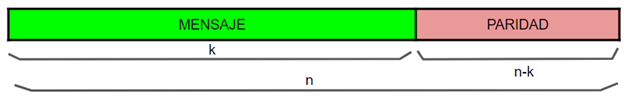
\includegraphics[scale=1]{Imagenes/Paridad.png}
	\label{fig:Paridad}
	%		\captionsetup{justification=raggedright,font={scriptsize,bf,it}}
	%		\caption*{fuente: http://superkuh.com/rtlsdr.html}
\end{figure}

\subsection{Los códigos convolucionales}

Pueden ser vistos como una variación de los códigos de bloques si se tiene en cuenta lo siguiente:

\begin{itemize}
    \item Tanto en los códigos de bloques como en los convolucionales, un mensaje se divide en bloques de bits o palabras que se pueden representar como $u_{2}, u_{1} , u_{0}$.
    \item En los códigos de bloques se usa una matriz \textbf{G}  que sirve de base para obtener la señal a transmitir, de modo que:
    \begin{equation} \label{capsiete_diesiocho}
    .... u_{2}, u_{1} , u_{0} \ \underrightarrow{G} \ (.... V_{2} = u_{2}G , v_{1} = u_{1}G, v_{0}=u_{0}G )
     \end{equation}
     \item En algunas fuentes se usa la representación polinomial que es la siguiente:
    \begin{equation} \label{capsiete_diesinueve}
    .... + u_{2} D^{2} +  u_{1}D + u_{0} \ \underrightarrow{G(D)} \ .... + u_{2}G D^{2} +  u_{1}GD + u_{0}G 
     \end{equation}
     \item Para el caso de los códigos convolucionales, lo que se tiene es una matriz para cada posición de la palabra de bits del mensaje $G_{0}$, $G_{1}$ , …,$G_{s}$ . También puede decirse que se tiene un polinomio de matrices: 
    \begin{equation} \label{capsiete_veinte}
    G_{0} \ + \ G_{1} + ... + \ G_{s} \ D^{s}
     \end{equation}
     Donde D puede ser visto como un retardo unitario (del inglés Delay). Osea que $G_{0}$ se aplica a la primera palabra del mensaje que llega, $G_{1}$ a la que llega con un retrazo, etc.
     \item De modo que, en la codificación convolucional, la señal a transmitir se calcula así:
    \begin{equation} \label{capsiete_veintiuno}
    (....u_{2},u_{1},u_{0}) \ \underrightarrow{G(D)} \ 
    (..., v_{2}= u_{2} G_{0} +u_{1}G_{1}+u_{0}G_{2},v_{1}=u_{1}G_{0}+u_{0}G_{1}),v_{0}=u_{0}G_{0}
     \end{equation}
     
     \item Como puede verse, cada palabra a transmitir, se obtiene usando varias palabras mientras se desplazan las matrices usadas, lo cual puede ser visto como una  convolución
     \item La representación polinomial para decir lo mismo anterior es la siguiente:
    \begin{equation} \label{capsiete_veintidos}
    ....+ u_{2}D^{2} \ + \ u_{1}D \ + \ u_{0} \ \underrightarrow{G(D)} \ 
    ... + (u_{2}G_{0} \ + \ u_{1}G_{1} \ + \ u_{0}G_{2})D^{2} \ + \ (u_{1}G_{0} \ + \ u_{0}G_{1})D + u_{0}G_{0}   )
     \end{equation}
     
     \item  Lo destacable de los códigos convolucionales es que una palabra a transmitir lleva información no solo de la palabra presente del mensaje sino también de palabras anteriores. Por ejemplo la palabra a transmitir $v_{2}$ se obtiene no solo a partir de la palabra del mensaje $u_{2}$ sino de $u_{1}$ y de $u_{0}$. Por eso se dice que los códigos convolucionales tienen memoria, es decir, guardan información de palabras transmitidas anteriormente.
\end{itemize}

Ejemplo de una matriz para un código convolucional.

\begin{equation} \label{capsiete_veintitres}
G(D)=\begin{bmatrix}
    D^{2}  \ + \ 1  \\
    D^{2} \ + \ D \  + \ 1   \\
\end{bmatrix}
     \end{equation}

Implementación para la anterior matriz \textcolor{blue}{\href{https://www.youtube.com/watch?v=8dIwK77czQI&feature=youtu.be&list=PLRuN7jX1rOZNj4gDf-eepcpaqCY3HjcaC&t=2375}{Vídeo}}

\subsection{Códigos binarios versus no binarios.}

\section{Técnicas de detección de errores}

\subsection{Chequeo de repeticiones.}

\subsection{Chequeo de paridad (Parity Check).}

Ha sido uno de los primeros métodos usados para detectar errores de un mensaje enviado desde un transmisor hasta un receptor pasando por un canal que puede producir interferencia y consecuentemente pérdidas de bits. En mensaje es visto de manera binaria, el mensaje a transmitir es visto como un bloque de bits, usualmente 8 bits, pero algunos de ellos, usualmente solo uno, el último, se destina para el proceso de control de paridad. \\

El proceso de insertar los bits de paridad:
\begin{itemize}
    \item Ocurre en el transmisor.
    \item contar el número de unos que hay en la información que se aloja en el bloque.
    \item Si el número de unos es impar, se agrega un uno en el espacio destinado al control de paridad, de lo contrario, en ese espacio se agrega un cero.
\end{itemize}

El proceso de control de errores:

\begin{itemize}
    \item Ocurre en el receptor.
    \item A cada bloque recibido se le cuentan los unos y siempre deberá dar un número par, de lo contrario, se habrá detectado un error \textcolor{blue}{\href{https://www.youtube.com/watch?v=pUBdJi6eVYA}{Vídeo}}
\end{itemize}

\subsection{Chequeo de polaridad}

\section{El mecanismo de corrección de Errores}

\subsection{Solicitud Automática de Repetición (ARQ)}

Solicitud automática de repetición (ARQ del inglés Automatic Repeat Request). Es la solución más obvia, donde la Corrección de errores se implementa como un sistema de solicitud de retransmisión parcial de la información.

\subsection{Corrección de Errores hacia adelante (FEC)}

Control de Errores hacia adelante (FEC del inglés Forward Error Correction). Consiste en la posibilidad de implementar la Corrección de errores como un proceso de recuperación de la información a partir de información redundante que ha sido emitida en el proceso de codificación realizado en el transmisor.
La Corrección de Errores hacia adelante (FEC del inglés Forward Error Correction) es una técnica usada en las comunicaciones digitales para darle la posibilidad al receptor de identificar un cierto número de errores en la señal de información recibida y corregirlos sin necesidad de recurrir a una retransmisión de la información, aunque a costa de usar un mayor ancho de banda en el canal. Por lo tanto es un elemento esencial en los sistemas de comunicación digital de tiempo real de voz, vídeo y otros servicios donde no resulta conveniente usar métodos de transmisión. \\

La idea central consiste en que el transmisor codifica el mensaje de una manera especial, usando cierta redundancia, para lo cual usa un Código de Corrección de Errores (ECC- Error Correcting Code). La idea fue presentada por primera vez en 1940 por el matemático americano Richard Hamming cuando inventó el ECC conocido como Hamming Code.
El ejemplo más sencillo es precisamente el Código de Repetición (3,1) explicado anteriormente.\\

Algunos codificadores FEC brindan la posibilidad de calcular la rata de errores de bit (BER del inglés Bit Error Ratio), lo cual resulta valioso para otros algoritmos de sintonización. \\

\section{Propiedades para la detección y corrección de Errores}

\textbf{Para la detección de errores:} Para detectar d errores de un bit entre dos palabras, es necesario un código con una distancia de Hamming de al menos d+1. Osea, que con una distancia de Hamming de d se pueden detectar d-1 errores.

\begin{itemize}
    \item Para corregir d errores de un bit entre dos palabras es necesario un código con una distancia de Hamming de al menos 2d+1. Osea que con una distancia de Hamming d se pueden corregir (d-1)/ errores. 
    \item Ejemplo C={0000000000,0000011111,1111100000}
    \item Distancia de Hamming =5
    \item Se pueden detectar d-1=4 errores
    \item Se pueden corregir (d-1)/2 = 2 errores 
\end{itemize}

Teorema básico de corrección de errores:

\begin{itemize}
    \item Un código C permite detectar hasta s errores si.
    
    \begin{equation} \label{capsiete_veinticuatro}
dist(C) \geq S+1
     \end{equation}
     
    \item Un código C permite corregir hasta t errorres si.
    \begin{equation} \label{capsiete_veinticinco}
dist(C) \geq 2t+1
    \end{equation}
     
\end{itemize}

\section{Códigos de redundancia cíclica (CRC)}

Código de chequeo de redundancia cíclica (CRC, del inglés - Cyclic and Redundancy Check).

\begin{itemize}
    \item Originalmente se tiene una secuencia de datos Por ejemplo: 1111111000000011110000000111
    \item Esa secuencia se divide en bloques de n elementos. Por ejemplo si n=7 y se continúa con el ejemplo anterior, se tienen 4 bloques cada uno con un espacio al final para agregar k elementos.


	\begin{table}[h!]
	    \captionsetup{justification = raggedright,singlelinecheck = false}
		\caption{Alguna descripción.}
		\label{tabla:tabla14}
				\centering
		\scalebox{1}{    
    \begin{tabular}{|l|l|l|l|l|l|l|l|l|l|l|l|l|l|l|l|l|l|l|l|l|l|l|l|l|}
    \hline
    \multicolumn{3}{|l|}{1111111} & \multicolumn{2}{l|}{} & \multicolumn{5}{l|}{0000000} & \multicolumn{2}{l|}{} & \multicolumn{3}{l|}{1111000} & \multicolumn{2}{l|}{} & \multicolumn{6}{l|}{0000111} & \multicolumn{2}{l|}{} \\ \hline
    \end{tabular}}
	\end{table}
	
    \item  Por eso se habla de un código tipo
        \begin{equation} \label{capsiete_veintiseis}
C(n,k)
    \end{equation}
    \item  El espacio en blanco a la derecha de cada bloque es para agregar información clave para facilitar la detección de errores. Esa información se deduce a partir un código binario que sea conocido tanto en el transmisor como en el receptor. A menudo no se habla de una palabra binaria en sí, sino de un polinomio generador de esa palabra.
\end{itemize}

\subsection {Proceso de codificación usando CRC}

\begin{itemize}
    \item El Proceso de codificación de una secuencia de datos  usando un Polinomio Generador G(x) en el transmisor es el siguiente:
\begin{itemize}
    \item Se selecciona el polinomio generador Por ejemplo $G(x)=x^{3}+1$
    \item Se prepara la secuencia de datos
Por ejemplo:\\ 
1111111\\ 
	Se supone que a ella le corresponde un polinomio que se puede representar como M(x).
    \item Tanto M(x) como G(x) se expresan como secuencias de bits.
    Para el ejemplo usado tenemos \\
$M(x) \rightarrow 1111111$ \\
$G(x) \rightarrow 1001$ \\
T(x) será el polinomio de la señal a transmitir \\
    \item Se agregan r ceros a la secuencia M(x), con lo cual se obtiene Q(x). Continuando con el ejemplo.\\
    $ Q(x) \rightarrow 1111111000$
    \item Se calcula el código CRC como el residuo que resulta al dividir G(x) por Q(x). Para nuestro ejemplo tenemos que: \\
$G(x)/Q(x)$ \\
1001 / 1111111000. \\

\begin{table}[h!]
	\centering
	\scalebox{1}{
\begin{tabular}{lllllllllll}
\multicolumn{5}{l}{$\oplus 1001$}   &  &    &      &     &     &    \\
   & \multicolumn{10}{l}{0110111000}                             \\
   & \multicolumn{5}{l}{$\oplus \underline{1001}$} &    &      &     &     &    \\
   &     & \multicolumn{9}{l}{010011000}                        \\
   &     & \multicolumn{9}{l}{$\oplus \underline{1001}$}                        \\
   &     &     & \multicolumn{8}{l}{00001000}                  \\
   &     &     &    &   &  & \multicolumn{5}{l}{$\oplus \underline{1001}$}      \\
   &     &     &    &   &  &    & \multicolumn{4}{l}{0001}
\end{tabular}}
\end{table}


El código CRC son las r últimas cifras del residuo, es decir 001 y se puede representar como R(x)
    \item Se determina el resultado o señal a transmitir T(x) adicionando el residuo obtenido en el punto anterior a Q(x). \\
    Para nuestro ejemplo $T(x) = Q(x)+R(x) $
    
    \begin{table}[h!]
	\centering
	\scalebox{1}{
    \begin{tabular}{rll}
    \multicolumn{3}{r}{1111111000} \\
    \multicolumn{3}{r}{$\underline{001}$}        \\
    \multicolumn{3}{r}{1111111\textcolor{red}{001}}
    \end{tabular}}
    \end{table}
   \item Vemos que finalmente T(x) es el mismo mensaje complementado con el código CRC.
    \end{itemize}
\end{itemize}

\subsection{Proceso de detección de errores usando Check sum}

Se realiza un proceso similar al visto en el proceso de codificación CRC. Si el residuo es 0 significa que no hay errores, de lo contrario hay errores. En calidad de ejemplo, veamos cómo se trataría la señal recibida del ejemplo anterior:


\begin{table}[h!]
	\centering
	\scalebox{1}{
\begin{tabular}{lllllrlllll}
\multicolumn{10}{l}{1111111\textcolor{red}{001}}                                       &  \\
\multicolumn{5}{l}{$ \oplus \underline{1001}$}         & \multicolumn{1}{l}{}  &  &  &  &  &  \\
 & \multicolumn{10}{l}{0110111001}                                       \\
 & \multicolumn{5}{l}{$ \oplus \underline{1001}$}                              &  &  &  &  &  \\
 &  & \multicolumn{8}{l}{010011001}                                   &  \\
 &  & \multicolumn{1}{r}{} & \multicolumn{3}{l}{$ \oplus \underline{1001}$}    &  &  &  &  &  \\
 &  &                      &  & \multicolumn{3}{l}{00001001} &  &  &  &  \\
 &  &                      &  &   & $ \oplus \underline{1001}$                 &  &  &  &  &  \\
 &  &                      &  &   & 0000                  &  &  &  &  & 
\end{tabular}}
\end{table}

En este ejemplo vemos que el residuo es cero, cuando la señal transmitida es idéntica a la recibida, es decir, cuando no se presentan errores. \\
Veamos un ejemplo, cuando se pierde un bit, por ejemplo cuando al receptor llega la señal: 1011111001

\begin{table}[h!]
	\centering
	\scalebox{1}{
\begin{tabular}{lllllrlllll}
\multicolumn{10}{l}{1011111001}                                       &  \\
\multicolumn{5}{l}{$ \oplus \underline{1001}$}         & \multicolumn{1}{l}{}  &  &  &  &  &  \\
 & \multicolumn{10}{l}{0010111001}                                       \\
 & \multicolumn{5}{l}{$ \oplus \underline{1001}$}                              &  &  &  &  &  \\
 &  & \multicolumn{8}{l}{00101001}                                   &  \\
 &  & \multicolumn{1}{r}{} & \multicolumn{3}{l}{$ \oplus \underline{1001}$}    &  &  &  &  &  \\
 &  &                      &  & \multicolumn{3}{l}{001101} &  &  &  &  \\
 &  &                      &  &   & $ \oplus \underline{1001}$                 &  &  &  &  &  \\
 &  &                      &  &   &  0100                  &  &  &  &  & 
\end{tabular}}
\end{table}

Vemos que se obtiene un residuo diferente de cero cuando la señal recibida es diferente a la transmitida.

\subsection{Cualidades del CRC}

\begin{itemize}
 \item detecta todos los errores de 1 bit.
 \item Si se escoje de manera apropiada G(x) se detecta.
 \item Todo error de 2 bits.
 \item Todo error de bits impares.
 \item Todo error de ráfagas con una longitud que es menor al grado r
 \item Es fácil de implementar en hardware binario.
 \item Es fácil de analizar matemáticamente.
 \item Es bueno para detectar errores comunes, causados por ruido en el canal de transmisión.
\end{itemize}

\section{La codificación de Reed Solomon}

Es uno de los tipos de codificación más notables ya que su uso se extendió al disco compacto (CD), el DVD, los discos duros, Blue-rays, otros sistemas de almacenamiento, los códigos QR, la televisión digital, WiMax, Comunicaciones satelitales, entre otros. Fue introducido en 1960 por Irving S. Reed y Gustave Solomon. 
Estrictamente pertenece al tipo de codificación cíclica no binaria y lo que hace es agregar t símbolos de chequeo a los datos para detectar cualquier combinación de hasta t símbolos erróneos o corregir hasta t/s símbolos
Este código tiene las siguientes cualidades:
\begin{itemize}
 \item Es un tipo de código linear sistemáticamente cíclico y es no-binario, usada en FEC. Desde este punto de vista, el chorro de datos del mensaje se divide en bloques de datos, se le agrega a estos bloques una redundancia que solo depende de las entradas actuales. 
 \item Se apoyan en un área de la matemática conocida como Campos de Galois o campos finitos. Estos campos se caracterizan por las operaciones aritméticas (+,-,x) siempre tienen un resultado dentro del campo. Precisamente, porque las herramientas de programación no soportan aritmética de campo de Galois, la implementación tradicional de este código es en hardware.
 \item Se representa como RS(n,k), 
 
 \begin{figure}[h!]
	\captionsetup{justification = raggedright, singlelinecheck = false}
	\caption{Codificación de Reed Solomon.} 
	\centering
	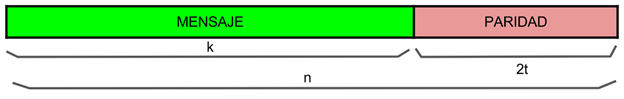
\includegraphics[scale=1]{Imagenes/RS.png}
	\label{fig:RS}
	%		\captionsetup{justification=raggedright,font={scriptsize,bf,it}}
	%		\caption*{fuente: http://superkuh.com/rtlsdr.html}
\end{figure}

donde: $n= 2^{s-1}$es la longittud del bloque resultante, s: es el número de bits que tiene cada simbolo del mensaje, k: es el número simbolos del mensaje en cada bloque, t es el número de simbolos erroneos que es posible corregir en la palabra del código. n es un número entero entre 3 y $2^{s}-1; k<n$, s es entero entre 3 y 16.
 \item Este código es capaz de corregir tanto errores en ráfagas como datos perdidos (erasures). Se usa principalmente en la corrección de ráfagas de errores.
 \item La ganancia de codificación de este código: es muy alta, aunque menor que los códigos LDPC y los TURBO códigos. Por esta alta ganancia, el código de Reed Solomon se usa en muchas aplicaciones incluyendo almacenamiento y transmisión de información:
 
 \begin{itemize}
 \item Almacenamiento (cintas de almacenamiento, discos compactos,DVD, etc).
 \item Comunicaciones móviles.
 \item Radioenlaces.
 \item Comunicaciones satelitales.
 \item Televisión digital
 \end{itemize}
 
 \item  La información puede estar dada en bits, pero también en bytes o en otro tipo de palabras. Por esa razón es ampliamente usada no solo en las comunicaciones sino también en sistemas de respaldo de información. Véase por ejemplo este \textcolor{blue}{\href{https://www.youtube.com/watch?v=jgO09opx56o}{Vídeo }}
\end{itemize}

El principio de la codificación consiste en:
 \begin{itemize}
 \item Se organiza la información en una matriz de dimensiones QxQ. \\
 
 Por ejemplo, si la información se organiza en una matriz 4x4 y está dada en bytes, en cierto momento podrían ser letras del alfabeto como en el siguiente caso:
 
$ U= \begin{bmatrix}
    A & B & C & D \\
    E & F & G & H \\
    I & J & K & L \\
    M & N & O & P
\end{bmatrix}$
 \item Contar con una matriz de dimensiones Qx(Q+k), donde el espacio QxQ de la matriz es una matriz de identidad y los demás espacios corresponden al código a usar.  \\
 
 Continuando con el ejemplo anterior, y teniendo en cuenta que la información está dada en bytes, la matriz puede ser la siguiente:
 
 $ G= \begin{bmatrix}
    01 & 00 & 00 & 00 \\
    00 & 01 & 00 & 00 \\
    00 & 00 & 01 & 00 \\
    00 & 00 & 00 & 01 \\
    1b & 1c & 12 & 14 \\
    1c & 1b & 14 & 12 
\end{bmatrix}$

 \item Se obtiene la matriz de la señal a transmitir como T=u x G.\\
 
 Continuando con el ejemplo, la información a transmitir está dada por la matriz siguiente:
 
  $ T \ = \ u \ x \ G = \begin{bmatrix}
    A & B & C & D \\
    E & F & G & H \\
    I & J & K & L \\
    M & N & O & P \\
    51 & 52 & 53 & 49 \\
    55 & 56 & 57 & 25 
\end{bmatrix}$

 \item Se toma la matriz obtenida y se transmite fila por fila. \\
 Continuando con el ejemplo anterior, la señal a transmitir es la siguiente:
 
\begin{table}[h!]
	\centering
	\scalebox{0.8}{
\begin{tabular}{llllllllllllllllllllllll}
\hline
\multicolumn{1}{|l|}{A} & \multicolumn{1}{l|}{B} & \multicolumn{1}{l|}{C} & \multicolumn{1}{l|}{D} & \multicolumn{1}{l|}{E} & \multicolumn{1}{l|}{F} & \multicolumn{1}{l|}{G} & \multicolumn{1}{l|}{H} & \multicolumn{1}{l|}{I} & \multicolumn{1}{l|}{J} & \multicolumn{1}{l|}{K} & \multicolumn{1}{l|}{L} & \multicolumn{1}{l|}{M} & \multicolumn{1}{l|}{N} & \multicolumn{1}{l|}{O} & \multicolumn{1}{l|}{P} & \multicolumn{1}{l|}{51} & \multicolumn{1}{l|}{52} & \multicolumn{1}{l|}{53} & \multicolumn{1}{l|}{49} & \multicolumn{1}{l|}{55} & \multicolumn{1}{l|}{56} & \multicolumn{1}{l|}{57} & \multicolumn{1}{l|}{25} \\ \hline
\multicolumn{16}{c}{$\underbrace{mensaje}$}                & \multicolumn{8}{c}{$\underbrace{paridad}$}                  \end{tabular}}
\end{table}
 El principio de la de-codificación, cuando no hay errores consiste en:
 \item Contar con una matriz que sea el inverso a la matriz usada para la decodificación. \\
 
 Para el ejemplo dado anteriormente, esa matriz es. 
  $ G^{-1}= \begin{bmatrix}
    01 & 00 & 00 & 00 \\
    00 & 01 & 00 & 00 \\
    00 & 00 & 01 & 00 \\
    00 & 00 & 00 & 01 \\
    8d & f6 & 7b & 01 \\
    f6 & 8d & 01 & 7b 
\end{bmatrix}$

 \item Se obtiene la señal recibida en forma matricial como $r = \ T \ X \ G^{-1} $

 \end{itemize}
 
 Cuando hay errores, la decodificación se realiza en 5 niveles:
 \begin{itemize}
 \item  Síndrome de cálculo: dice si ocurrió un error  durante la transmisión de datos
 \item Localización del error: dice donde se presentó el error
la magnitud del error
 \item Evaluación del error: corrige el error.
 \end{itemize}
 
 Tres son los posibles resultados de la decodificación:
 \begin{itemize}
 \item  Si $2s + r < 2t$ , donde s son símbolos con errores, r son símbolos borrados, entonces la palabra de código originalmente transmitida podrá ser siempre recuperada
 \item El decodificador detectará que no puede recuperar la palabra de código original e indicará  este hecho.
 \item El decodificador decodificará erróneamente y recuperará una palabra de código de manera incorrecta y sin indicación alguna.
 \end{itemize}
 
 Otras aplicaciones de la codificación Reed Solomon. \\

Los métodos de codificación pueden encontrar una gran cantidad de aplicaciones. 

\begin{table}[h!]
	\centering
	\scalebox{0.65}{
\begin{tabular}{|l|l|l|l|l|l|l|l|l|l|l|l|l|l|l|l|l|l|l|l|l|l|l|l|}
\hline
\multicolumn{24}{|l|}{Ejemplo aplicado a bases de datos. El mismo ejemplo anterior, aplicado al respaldo de bases de datos se encuentra en el siguiente vídeo:} \\
\multicolumn{24}{|l|}{\textcolor{blue}{\href{https://www.youtube.com/watch?v=jgO09opx56o}{Codificador Reed Solomon aplicado para el respaldo de bases de datos}}}                                              \\
\multicolumn{24}{|l|}{}                                              \\
\multicolumn{24}{|l|}{Hay también una gran multitud de aplicaciones como es el caso de los QR Codes:}                                              \\
\multicolumn{24}{|l|}{\textcolor{blue}{\href{https://www.youtube.com/watch?v=hNWBqE5f_pY}{Reed Solomon aplicado a Códigos QR}}}                                              \\ \hline
\end{tabular}}
\end{table}

\section{Reed Solomon RS(255,223)en la práctica}

En la práctica es común encontrar una configuración del Reed Solomon, donde cada  palabra de código que se produce es de 255 bytes, de los cuales k=223 son bytes del mensaje y 2t=32 son bytes de paridad: \\
n=255, \\
k=223, \\
consecuentemente, s=8, \\
2t=32, \\
t=16 \\
Eso indica que este código permite corregir  hasta 16 símbolos erróneos en la palabra de código, en cualquier parte del código y de manera automática. \\

\vspace{600px}
\section{Modelo de capas de DVB-T}

 \begin{figure}[h!]
	\captionsetup{justification = raggedright, singlelinecheck = false}
	\caption{Modelo de capas de la capa física de dvb-t.} 
	\centering
	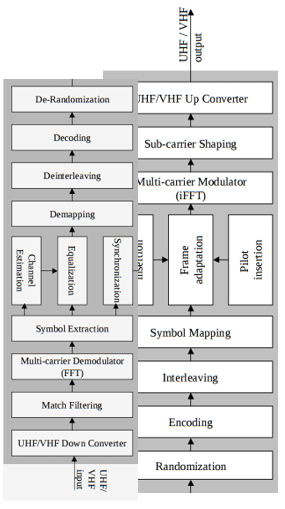
\includegraphics[scale=1]{Imagenes/UHF-VHF.png}
	\label{fig:UHF-VHF}
		\captionsetup{justification=raggedright,font={scriptsize,bf,it}}
			\caption*{fuente:  ETSI EN 301 958}
\end{figure}

\section{Scrambling en DVB-T}

El scrambling es un tema que ya ha sido explicado en el capítulo 1. Para el caso de la DVB-T el scrambling tiene las siguientes particularidades:

 \begin{itemize}
 \item  La secuencia PN se genera mediante una interconexión de 15 registros, una compuerta XOR y una AND.
 \vspace{200px}
  \begin{figure}[h!]
	\captionsetup{justification = raggedright, singlelinecheck = false}
	\caption{Esquema de scrambling} 
	\centering
	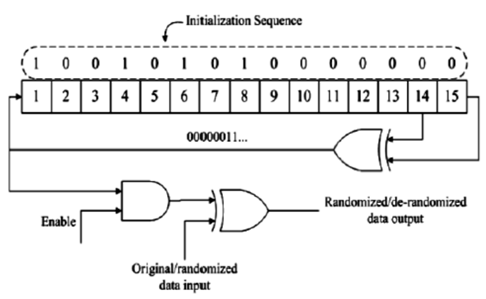
\includegraphics[scale=1]{Imagenes/Esquema-scrambling.png}
	\label{fig:Esquema-scrambling}
	%	\captionsetup{justification=raggedright,font={scriptsize,bf,it}}
	%		\caption*{fuente:  ETSI EN 301 958}
\end{figure}

 \item. Esta interconexión puede entenderse con la teoría que se explica en el libro de Haykin, capítulo 7, sobre generación de señales PN.
 \item Los registros están conectados en serie y con cada pulso de reloj, el estado de un registro pasa al siguiente registro.
\item Los estados de los registros son los de la secuencia de inicialización que aparece en la figura, cuyo polinomio generador es $p(x) = 1+x^{14}+x^{15}$
\item El esquema es equivalente a la Fig. 1, pero si bs(t) se cambia de polaridad, osea que se multiplica por -1.
\item Los registros 14 y 15 entregan su estado a una compuerta XOR y su salida va pasando nuevamente al primer registro y al mismo tiempo a una compuerta AND. 
\item El scrambling ocurre en una compuerta XOR, a la cual entran el código PN y la señal útil.
\item El periodo que resulta para la secuencia PN es de 188*8=12032 bits.
\item El primer byte de cada paquete de la señal de video es de sincronización y no debe ser aleatorizado. Sin embargo el generador PN sigue generando bits aunque no se usen en esos bytes específicos. Justamente, la entrada Enable es la que desactiva o activa el scrambling para estos casos. La entrada Enable puede ser vista como un vector cuyos bits cambian cuando es necesario detener el scrambling.
 \end{itemize}
 
 \section{FEC en DVB-T}